\chapter{Firewall and IDS/IPS}
\cite{05_Firewalling}

\section*{What is a Firewall?}
Literally, a firewall is a ‘wall to protect against fire propagation’ (a safety feature designed to compartmentalize fire and limit damage). In the context of computer networks, it guarantees a controlled connection between networks at different security levels, serving as boundary protection and a network filter.

\section{Ingress vs. Egress Firewall}
\begin{tcolorbox}[colback=red!10!white, colframe=red!70!black, coltitle=white, title=Beware]
    Bidirectional protection is essential. This concept involves protecting both incoming (ingress) and outgoing (egress) network traffic to ensure comprehensive security.
\end{tcolorbox}

\textbf{The Ingress Firewall:}
\begin{itemize}
    \item Is intended for \textbf{incoming} connections.
    \item Typically, \textbf{controls access} to the (public) services offered by your network or system.
\end{itemize}

\textbf{The Egress Firewall:}
\begin{itemize}
    \item Is intended for \textbf{outgoing} connections.
    \item Typically, used to \textbf{monitor and control} the activity of internal personnel or devices (to prevent unauthorized traffic, and also for privacy and data protection).
\end{itemize}

\begin{tcolorbox}[colback=blue!10!white, colframe=blue!50!white, title=Classification of Traffic]
    It’s straightforward to classify traffic for \textbf{channel-based services} (e.g., TCP applications), but more challenging for \textbf{message-based stateless services} (e.g., ICMP, UDP applications), due to their lack of a consistent connection state.
\end{tcolorbox}

\section{Three Commandments of Firewall}
\begin{center}
    1. The firewall (FW) must be the only contact point between the internal network and the external network.
\end{center}

\begin{center}
    2. Only “authorized” traffic should be allowed to pass through the firewall.
\end{center}

\begin{center}
    3. The firewall must be a highly secure system.
\end{center}

\emph{-- D. Cheswick and S. Bellovin}

\noindent Referring to each rule:
\begin{enumerate}
    \item The behavior of employees poses a risk.
    \item The technician must understand what they are configuring, especially which rules are necessary.
    \item Dedicated security elements should be used to avoid cross-vulnerabilities.
\end{enumerate}

\section{Authorization Policies}
We have two possible choices:
\begin{itemize}
    \item \textbf{Permitlist} (AKA allowlist): "All that is not explicitly permitted, is forbidden."
    \begin{itemize}
        \item Higher security (gatekeeper).
        \item More complex to manage.
    \end{itemize}
    \item \textbf{Blocklist} (AKA denylist): "All that is not explicitly forbidden, is permitted."
    \begin{itemize}
        \item Lower security (open gates).
        \item Easier to manage.
    \end{itemize}
\end{itemize}

\section*{FW: Basic Components}
\begin{tcolorbox}[colback=red!10!white, colframe=red!70!black, coltitle=white, title=Beware]
The Firewall is a system! With several components.
\end{tcolorbox}

\begin{itemize}
    \item \textbf{Packet filter / screening router / choke}: A component that filters traffic at the network level.
    \item \textbf{Bastion host}: A secure system with auditing.
    \item \textbf{Application gateway (proxy)}: A service that works on behalf of an application, with access control.
    \item \textbf{Dual-homed gateway}: A system with two network cards and routing disabled (ip-forwarding off).
\end{itemize}

\begin{tcolorbox}[colback=blue!10!white, colframe=blue!50!white, title=What is a Proxy]
    A proxy is a system or service that sits between the client and the application server. It intercepts and controls the traffic between the two, often for purposes such as filtering, caching, security, or access control. A proxy is not inherently a firewall, but it can function in a way similar to a firewall depending on its role and how it’s configured.
\end{tcolorbox}

\section{Control Mechanisms for each Level}
To provide a clear and structured explanation of the different controls at various network levels, here’s an overview of each control type along with a comparison of how they differ in terms of:
\begin{itemize}
    \item Controls to be performed (i.e., threats detected).
    \item Performance.
    \item Protection of the firewall OS.
    \item Keeping or breaking the client-server model (where breaking means no direct communication between client and server).
\end{itemize}

\noindent Different controls at various network levels:
\begin{itemize}
    \item (Static) packet filter.
    \item Stateful/stateless (dynamic) packet filter.
    \item Cutoff proxy.
    \item Circuit-level gateway / proxy.
    \item Application-level gateway / proxy.
    \item Stateful inspection.
\end{itemize}

\begin{figure}[H]
  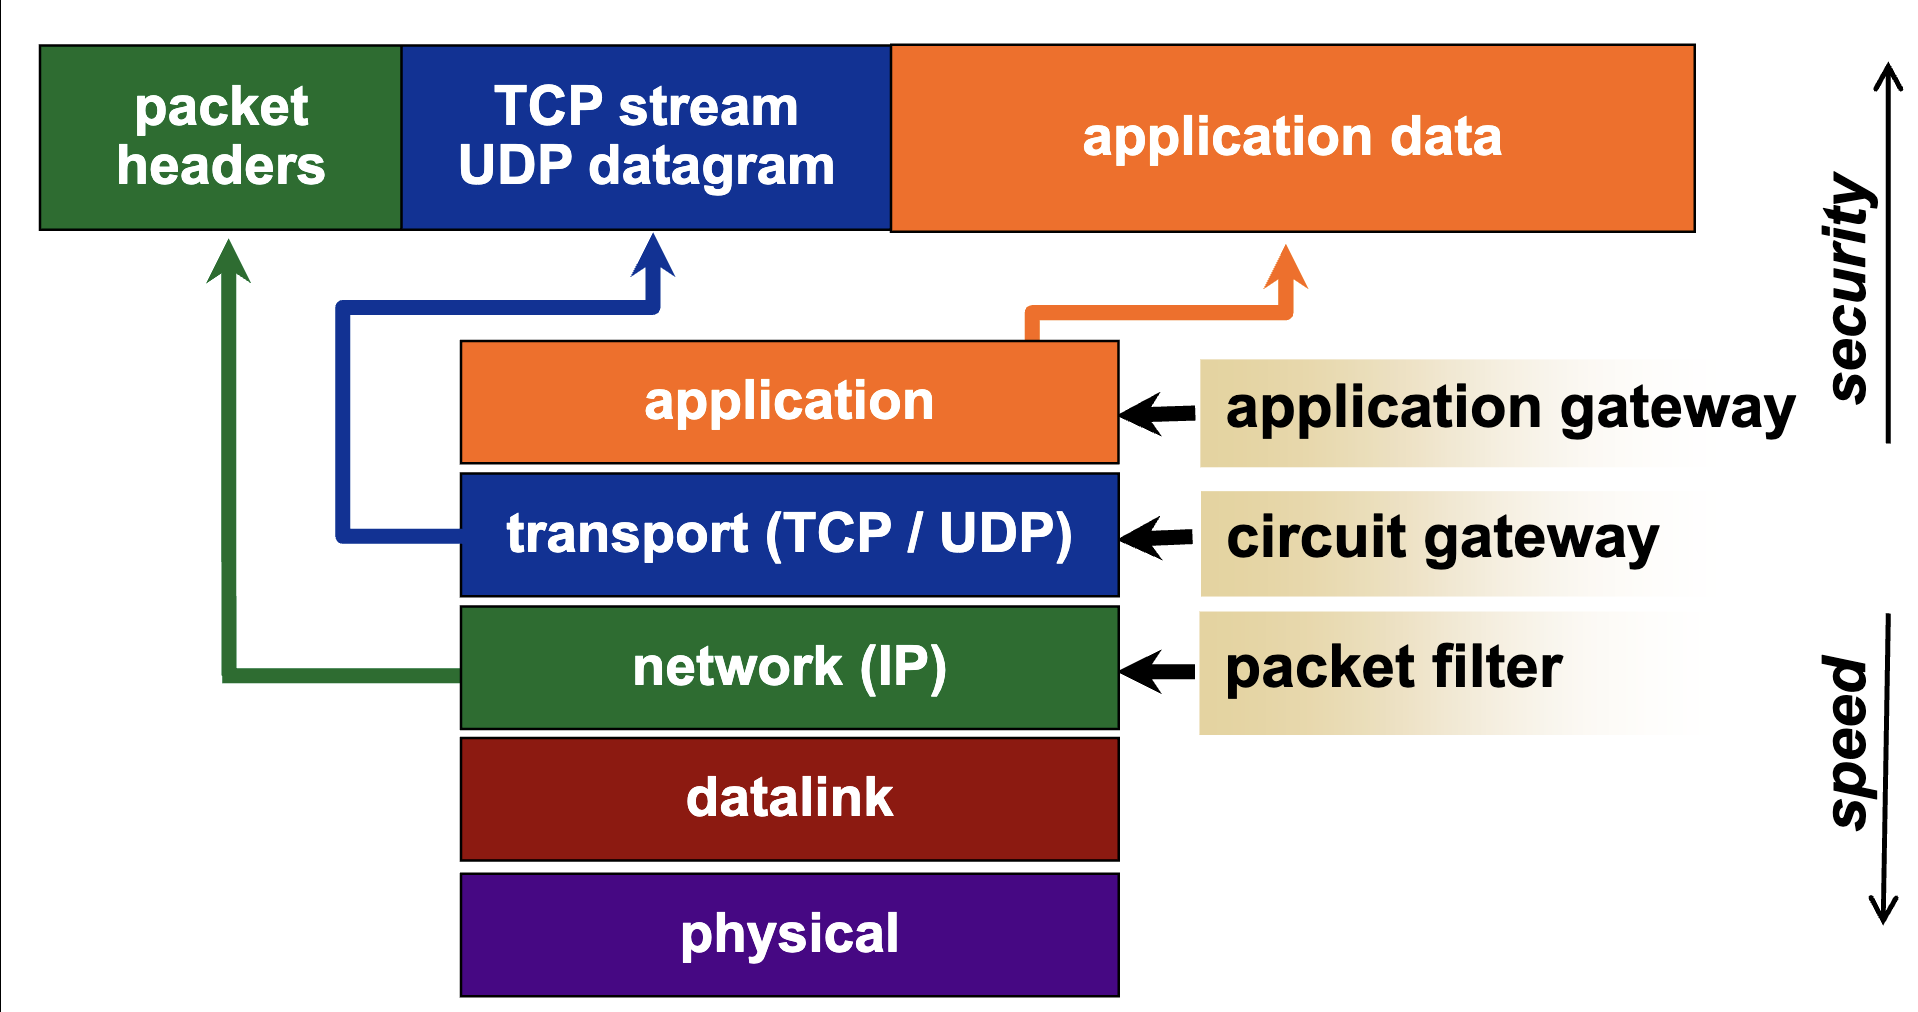
\includegraphics[width=\linewidth]{Images/Firewalling/levels.png}
  \caption{Controls for each level.}
\end{figure}

\subsection{Packet Filter}
\begin{tcolorbox}[colback=red!10!white, colframe=red!70!black, coltitle=white, title=Beware]
    Order is important (first match principle).
\end{tcolorbox}
\begin{itemize}
    \item Historically available on routers, nowadays found in almost every OS.
    \item Performs packet inspection at the network level.
    \item Inspects the IP header.
    \item Inspects the transport header.
    \item Rule examples:
    \begin{itemize}
        \item Permit incoming connections to our web server:
        \begin{quote}
            \texttt{src any dst 10.1.2.3/0.0.0.0 tcp 80 allow}
        \end{quote}
        \item Only our internal DNS server can query external DNS servers:
        \begin{quote}
            \texttt{src 10.1.2.1/0.0.0.0 dst any udp 53 allow}
        \end{quote}
    \end{itemize}
\end{itemize}

\begin{itemize}
    \item \textbf{Pros:}
    \begin{itemize}
        \item Independent of applications.
        \item Good scalability.
        \item Good performance.
        \item Low cost (available on routers and in many OS).
    \end{itemize}
    \item \textbf{Cons:}
    \begin{itemize}
        \item Approximate controls: easy to "fool" (e.g., IP spoofing, fragmented packets).
        \item Difficult to support services with dynamically allocated ports (e.g., FTP).
        \item Complex to configure (and understand the configuration sometimes).
        \item Difficult to perform user authentication.
    \end{itemize}
\end{itemize}

\subsection{Circuit-level Gateway}
\textbf{Generic Proxy (i.e., not "Application-Aware")}
\begin{itemize}
    \item Creates a transport-level circuit between the client and server.
    \item Does not understand or manipulate the payload data in any way.
    \item Simply copies TCP segments or UDP datagrams between its two interfaces, provided they match the access control rules.
    \item Re-assembles the IP packets, which helps provide protection against some Layer 3 (L3) and Layer 4 (L4) attacks.
    \item Breaks the TCP/UDP-level client/server model during the connection.
    \item Provides more protection for the server.
    \begin{itemize}
        \item Isolated from attacks related to the TCP handshake.
        \item Isolated from attacks related to IP fragmentation.
    \end{itemize} 
    \item May authenticate the client, but this requires modification to the application.
    \item Exhibits many limitations of a packet filter.
    \item \textbf{SOCKS} is one of the most well-known examples of a generic proxy.
\end{itemize}

\subsection{Application-level Gateway}
Composed of a set of proxies (collection of elements) inspecting the packet payload at the application level:
\begin{itemize}
    \item Often requires modifications to the client application.
    \item May optionally mask or renumber the internal IP addresses.
    \item When used as part of a firewall, usually performs peer authentication.
    \item Provides top security (e.g., protects against buffer overflow vulnerabilities in the target application).
    \item Difference between forward proxy (egress) and reverse proxy (ingress).
    \item Rule example:
    \begin{quote}
        \texttt{deny dangerous HTTP methods "PUT, DELETE deny"}
    \end{quote}
    \item SMP (Symmetric Multiprocessing) may improve performance.
\end{itemize}

\begin{itemize}
    \item \textbf{Pros:}
    \begin{itemize}
        \item Rules are more fine-grained and simpler compared to those of a packet filter.
        \item Provides more protection for the server.
        \item May authenticate the client.
    \end{itemize}
    \item \textbf{Cons:}
    \begin{itemize}
        \item Every application requires a specific proxy.
        \item Delay in supporting new applications.
        \item Heavy on resources (many processes).
        \item Low performance (due to user-mode processes).
        \item Completely breaks the client/server model.
        \item Not transparent to the client.
        \item The proxy's OS may be vulnerable to attacks.
        \item Problems with Application-Level Security Techniques that Do Not Permit Traffic Inspection (e.g., TLS)
    \end{itemize}
\end{itemize}

\textbf{Variants of Application-level Gateway:}
\begin{itemize}
    \item \textbf{Transparent Proxy:}
    \begin{itemize}
        \item Less intrusive for the client.
        \item Requires additional work (packet rerouting and destination extraction).
    \end{itemize}
    \item \textbf{Strong Application Proxy:}
    \begin{itemize}
        \item Checks semantics, not just syntax.
        \item Only some commands/data are forwarded, based on deeper inspection.
        \item This is the only correct configuration for a proxy in cases requiring high security.
    \end{itemize}
\end{itemize}

\subsection*{HTTP Proxy}
\begin{center}
    \textbf{Forward Proxy}
\end{center}

\begin{itemize}
\item {HTTP Server Acting as a Front-End:}
\item Acts as an egress control, passing requests to the real (external) server.
\item \textbf{Benefits} (in addition to network ACLs):
\begin{itemize}
    \item Shared cache of external pages for all internal users.
    \item Authentication and authorization of internal users.
    \item Various controls, such as allowed sites, transfer direction, data types, etc.
\end{itemize}
\end{itemize}

\begin{figure}[H]
    \centering
    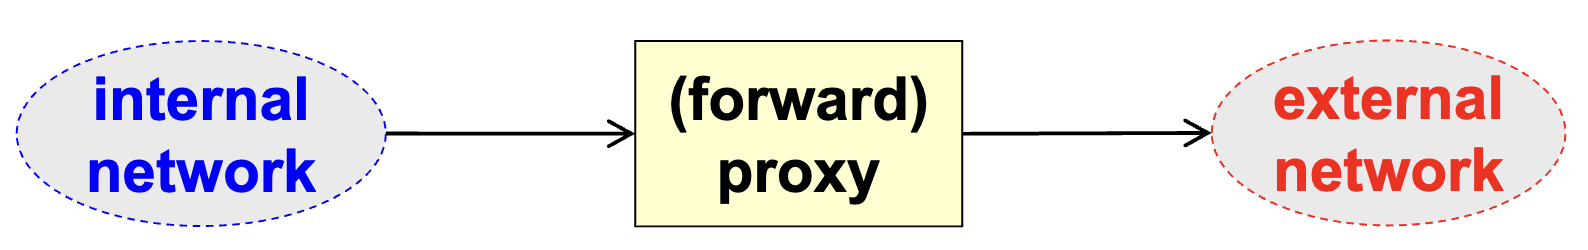
\includegraphics[width=0.5\linewidth]{Images/Firewalling/forward_proxy.png}
    \caption{Forward proxy example.}
\end{figure}
    
\begin{center}
    \textbf{Reverse Proxy}
\end{center} 

\begin{itemize}
    \item Acts as a front-end for the real server(s), forwarding requests to them.
    \item Implements network ACL and content inspection.
    \item \textbf{Additional Benefits:}
    \begin{itemize}
        \item Obfuscation: Hides information about the real server(s).
        \item TLS Accelerator: Handles TLS encryption, leaving unprotected connections between the proxy and the backend servers.
        \item Load Balancer.
        \item Web Accelerator: Caches static content.
        \item Compression.
        \item Spoon Feeding: Retrieves a full dynamic page from the backend server and delivers it to the client based on its speed, offloading the application server.
    \end{itemize}
\end{itemize}

\begin{figure}[H]
    \centering
    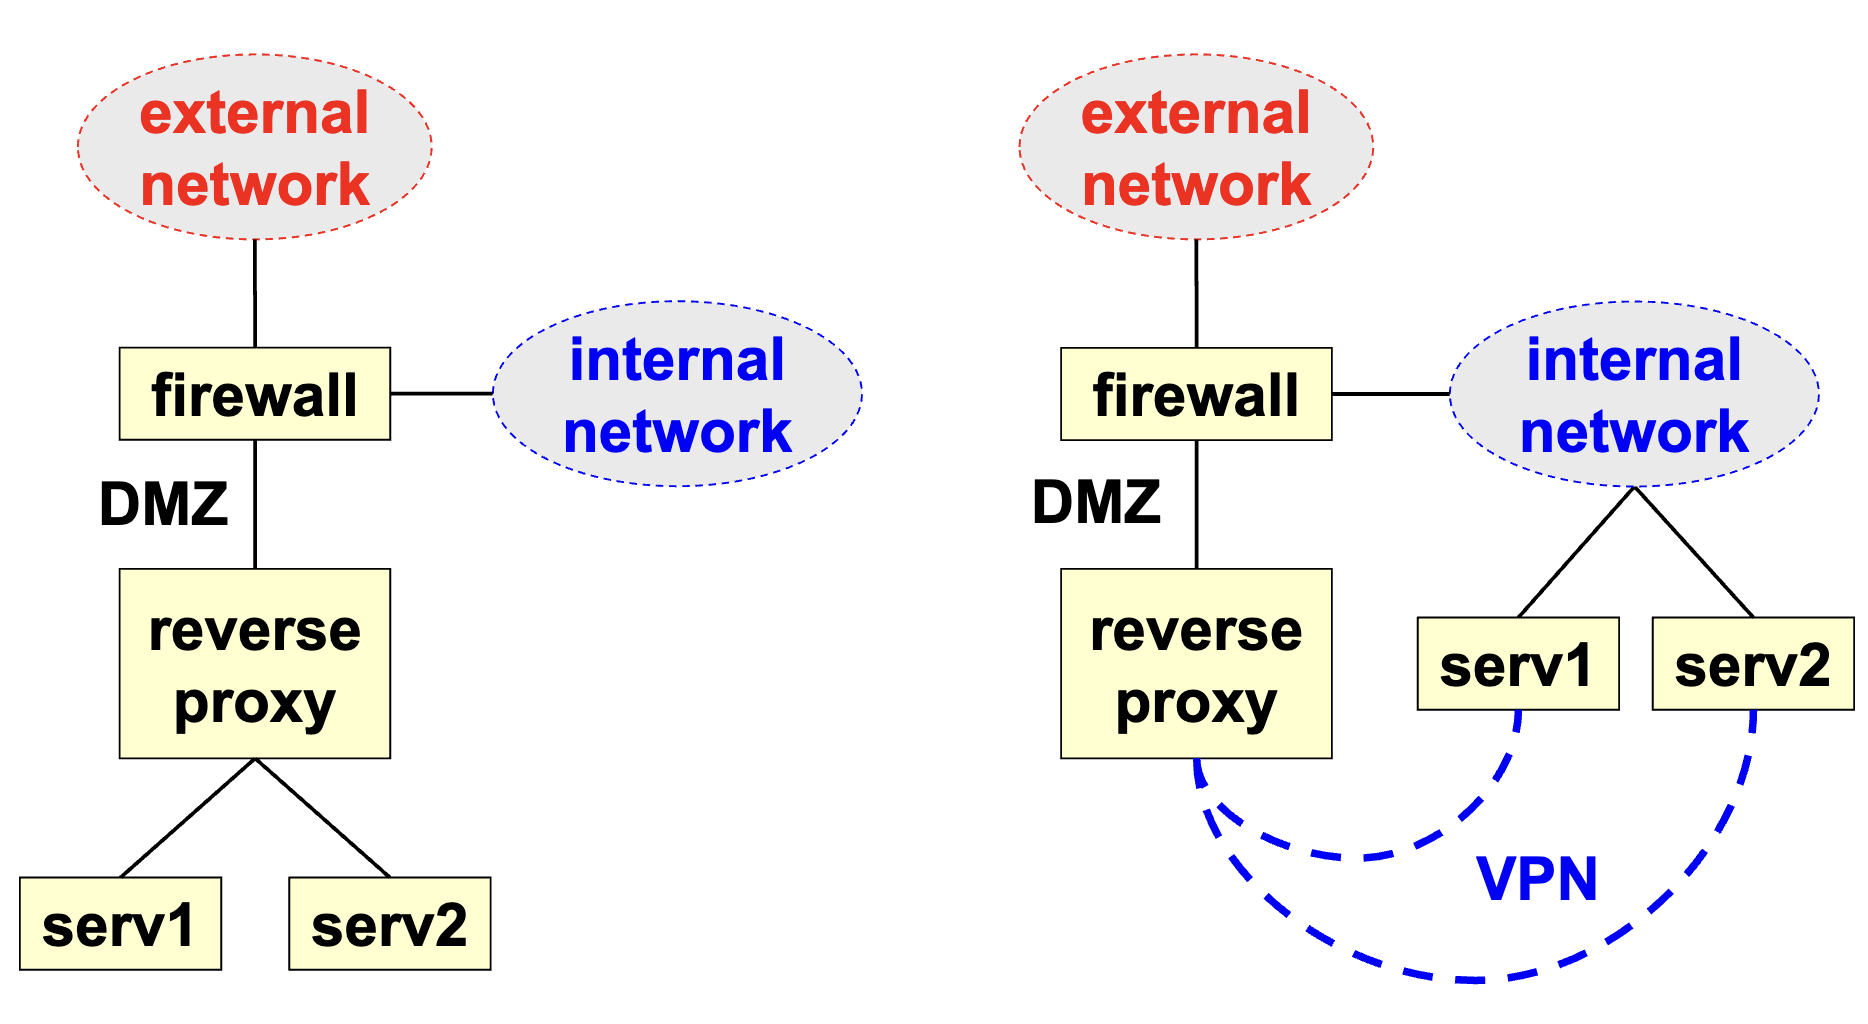
\includegraphics[width=0.5\linewidth]{Images/Firewalling/reverse_proxy.png}
    \caption{Reverse proxy example.}
\end{figure}

\subsection{WAF}
\begin{center}
(Web Application Firewall)
\end{center}

\begin{tcolorbox}[colback=blue!10!white, colframe=blue!50!white]
    The implementation of this module enables a proxy to function as an application firewall.
\end{tcolorbox}

The large use of web applications leads to an increase in threats targeting them.
\begin{itemize}
    \item A WAF is a module installed at a proxy (either forward and/or reverse) to filter application traffic.
    \item Filters the following types of traffic:
    \begin{itemize}
        \item HTTP commands.
        \item HTTP request/response headers.
        \item HTTP request/response content.
    \end{itemize}
    \item \textbf{ModSecurity:}
    \begin{itemize}
        \item A popular plugin for Apache and NGINX, which power about 50\% and 30\% of worldwide HTTP servers, respectively.
        \item Includes the \textbf{OWASP ModSecurity Core Rule Set (CRS)} to protect against a wide range of attacks.
    \end{itemize}
\end{itemize}

\section{Firewall Architectures}
\subsection{Packet Filter}
Control the flow of traffic between networks or network segments. It operates at the network layer (Layer 3) inspecting each packet’s header and making decisions based on predefined filtering rules. The architecture of a packet filter is designed to act as a firewall that filters traffic based on IP addresses, protocols, ports, and other packet header attributes, without inspecting the payload data.

\begin{tcolorbox}[colback=red!10!white, colframe=red!70!black, coltitle=white, title=Beware]
    Simple, cost-effective, but... insecure!
\end{tcolorbox}

\begin{itemize}
    \item Exploits the packet filter to screen traffic at both the IP and upper layers.
    \item The Packet Filter element represents a single point of failure.
    \item If implemented with a router, it becomes a "screening router," eliminating the need for additional dedicated hardware.
    \item No need for a proxy, thus no modification of applications is required.
\end{itemize}

\begin{figure}[H]
    \centering
    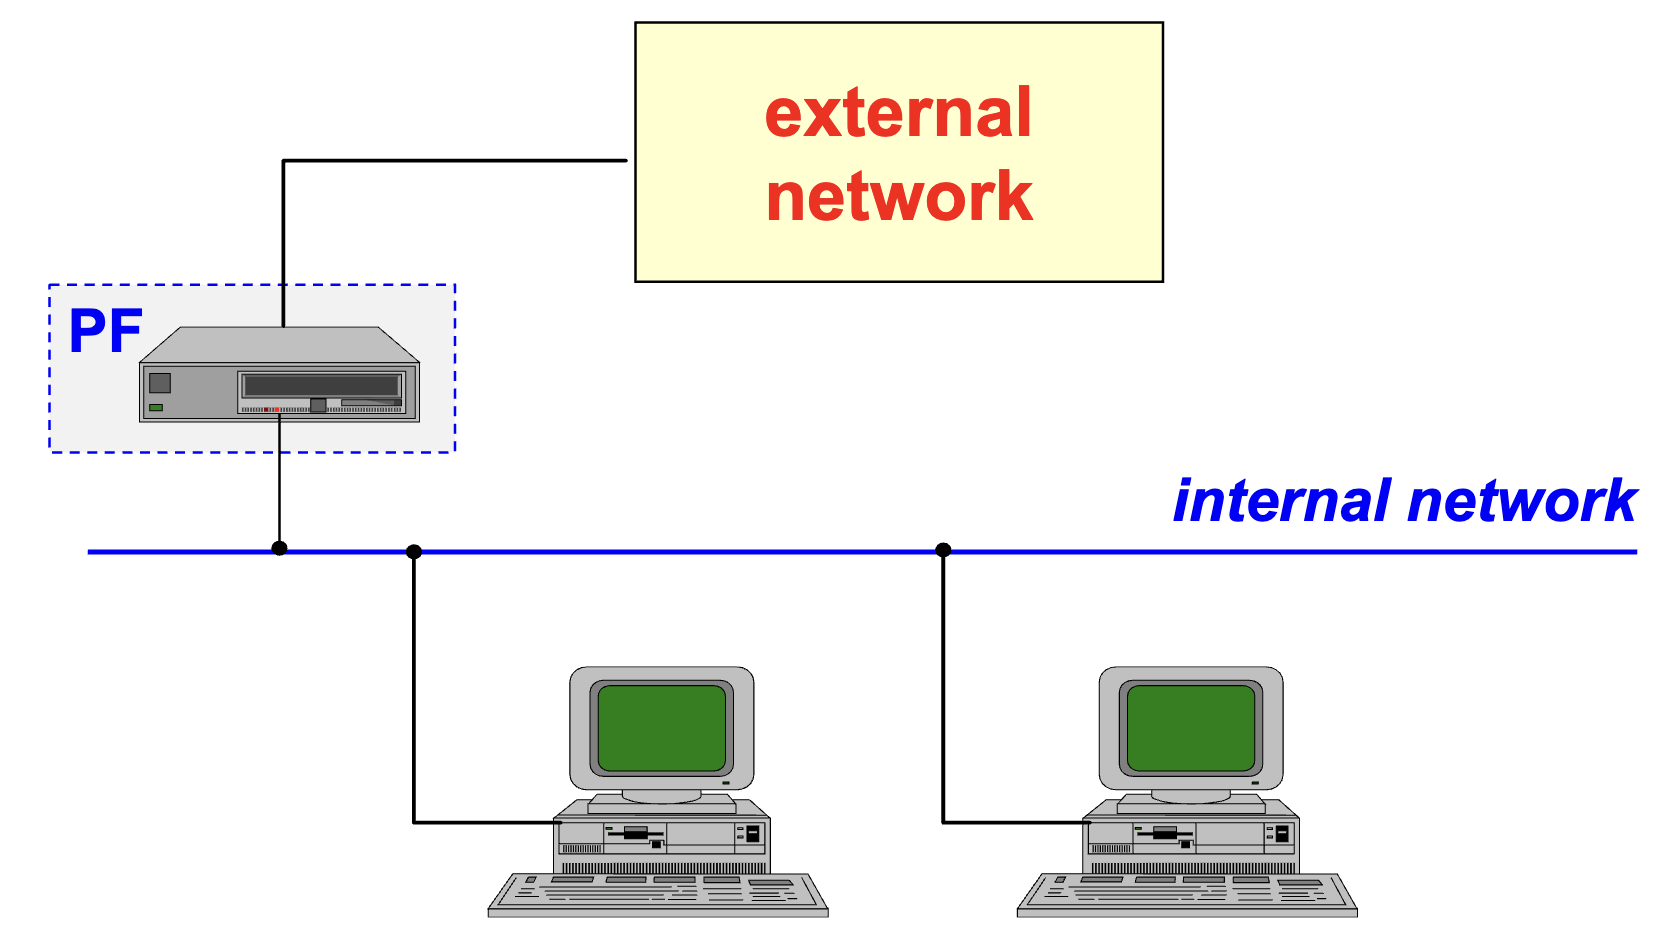
\includegraphics[width=0.5\linewidth]{Images/Firewalling/packet_filter.png}
    \caption{Packet filter architecture.}
\end{figure}

\subsection{Dual-homed Gateway}
A Dual-Homed Gateway uses a bastion host with two NICs (Network Interface Cards) to connect to two different networks, typically a trusted internal network and an untrusted external network (such as the internet). This configuration provides a layer of security by isolating and controlling the communication between the two networks.

\begin{itemize}
    \item Easy to implement.
    \item Small additional hardware requirements.
    \item The internal network can be masqueraded.
    \item Inflexible: The packet filter cannot easily adapt to changing network requirements or policies, and it does not provide much flexibility in managing traffic.
    \item High work overhead.
    \item The border router performs an initial screening of the traffic.
    \item The bastion host (gateway) could become a bottleneck, reducing the overall performance of the system.
\end{itemize}

\begin{figure}[H]
    \centering
    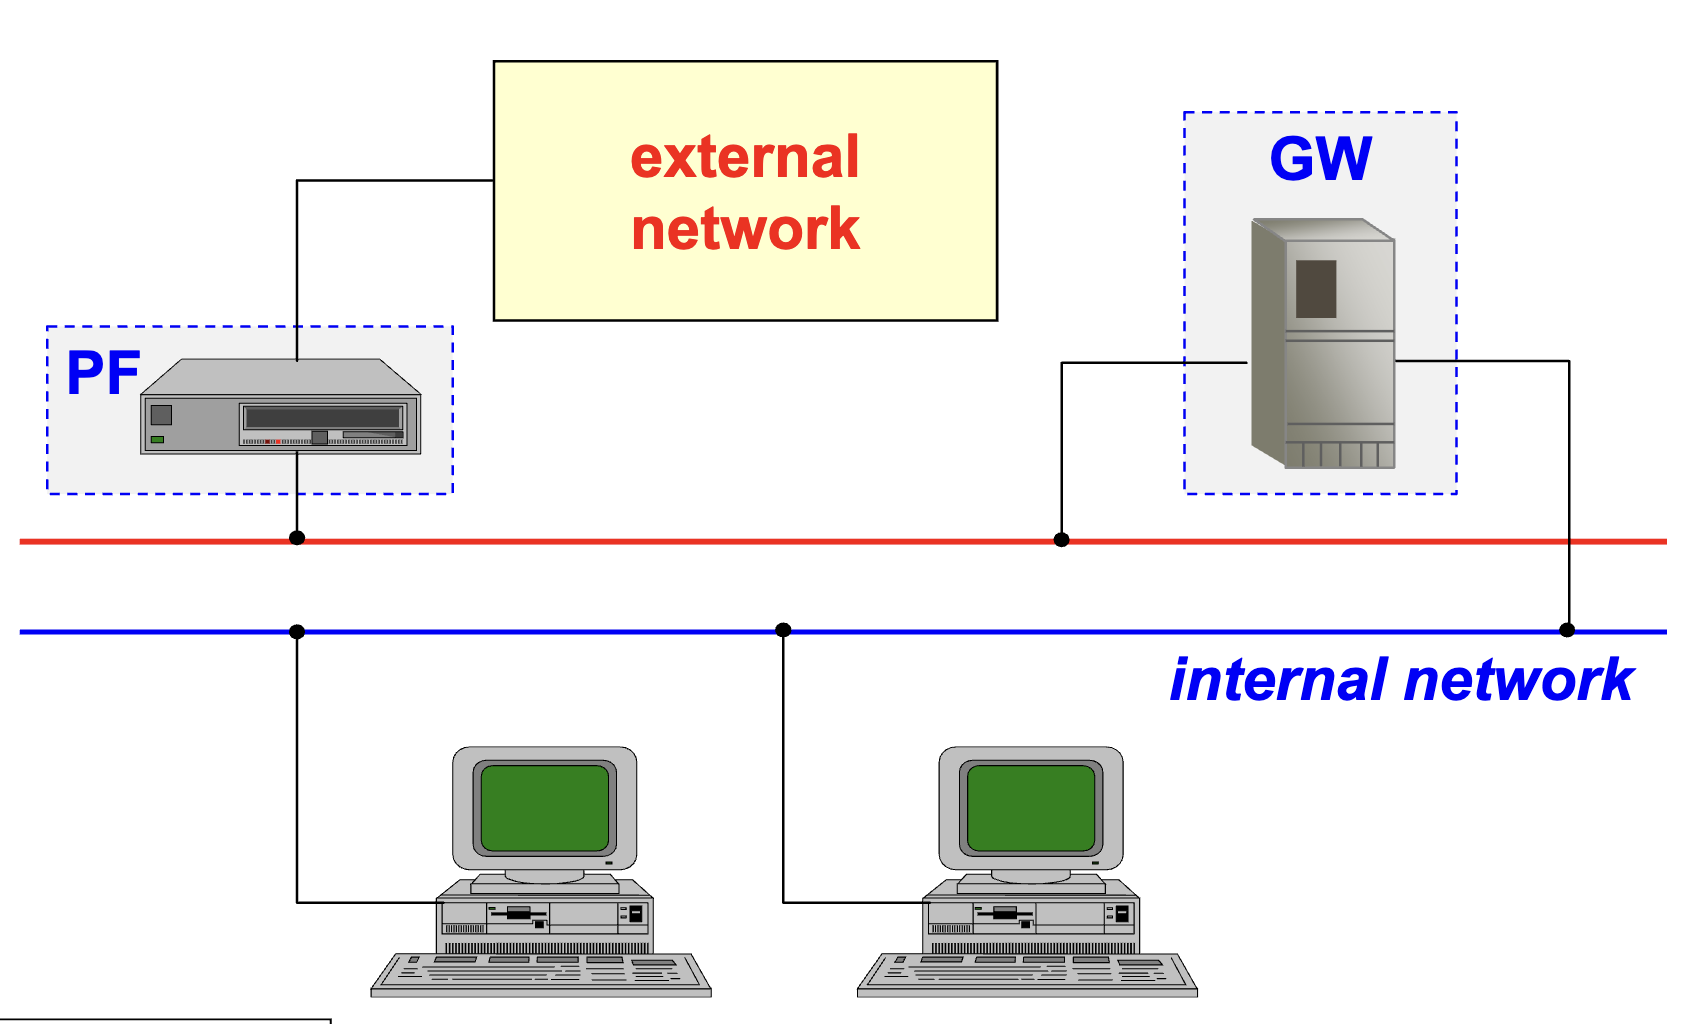
\includegraphics[width=0.5\linewidth]{Images/Firewalling/dual_homed_gateway.png}
    \caption{Dual-homed gateway architecture.}
\end{figure}

\subsection{Screened Host}
Uses two primary components: a router and a bastion host. This setup aims to provide enhanced security by controlling the flow of traffic between the internal and external networks. Below are the characteristics and key features of this architecture:

\begin{itemize}
    \item Router:
    \begin{itemize}
        \item Acts as a filtering device between the internal (INT) and external (EXT) networks.
        \item Blocks traffic from internal to external networks (INT > EXT) unless the traffic is coming from the bastion host.
        \item Blocks traffic from external to internal networks (EXT > INT) unless it is directed towards the bastion host.
        \item Exceptions: The router allows traffic for directly enabled services, meaning services that are explicitly allowed (e.g., HTTP, DNS) can pass through based on predefined rules.
    \end{itemize}
    \item Bastion Host:
    \begin{itemize}
        \item Serves as a secure intermediary and runs either a circuit gateway or an application gateway.
        \item Controls access to the authorized services (e.g., web servers, FTP servers) by inspecting and filtering traffic at a deeper level.
        \item Ensures that only legitimate services are accessible to the external network, protecting the internal network from unauthorized access.
    \end{itemize}
    \item Pros and Cons:
    \begin{itemize}
        \item More Expensive and Complex to Manage: The setup is more complex because it involves managing two systems (router + bastion host), which increases both the cost and administrative overhead.
        \item More Flexible: The architecture offers flexibility because it allows skipping control over some services or hosts. For example, some services may bypass the bastion host if specifically configured to do so, making it easier to manage certain use cases.
        \item Limited Masking: Only the hosts and protocols that go through the bastion host can be masked for security (such as hiding internal IP addresses or data). However, if the packet filter (PF) uses NAT (Network Address Translation), it can mask additional traffic and hide internal network details.
    \end{itemize}
\end{itemize}

\begin{figure}[H]
    \centering
    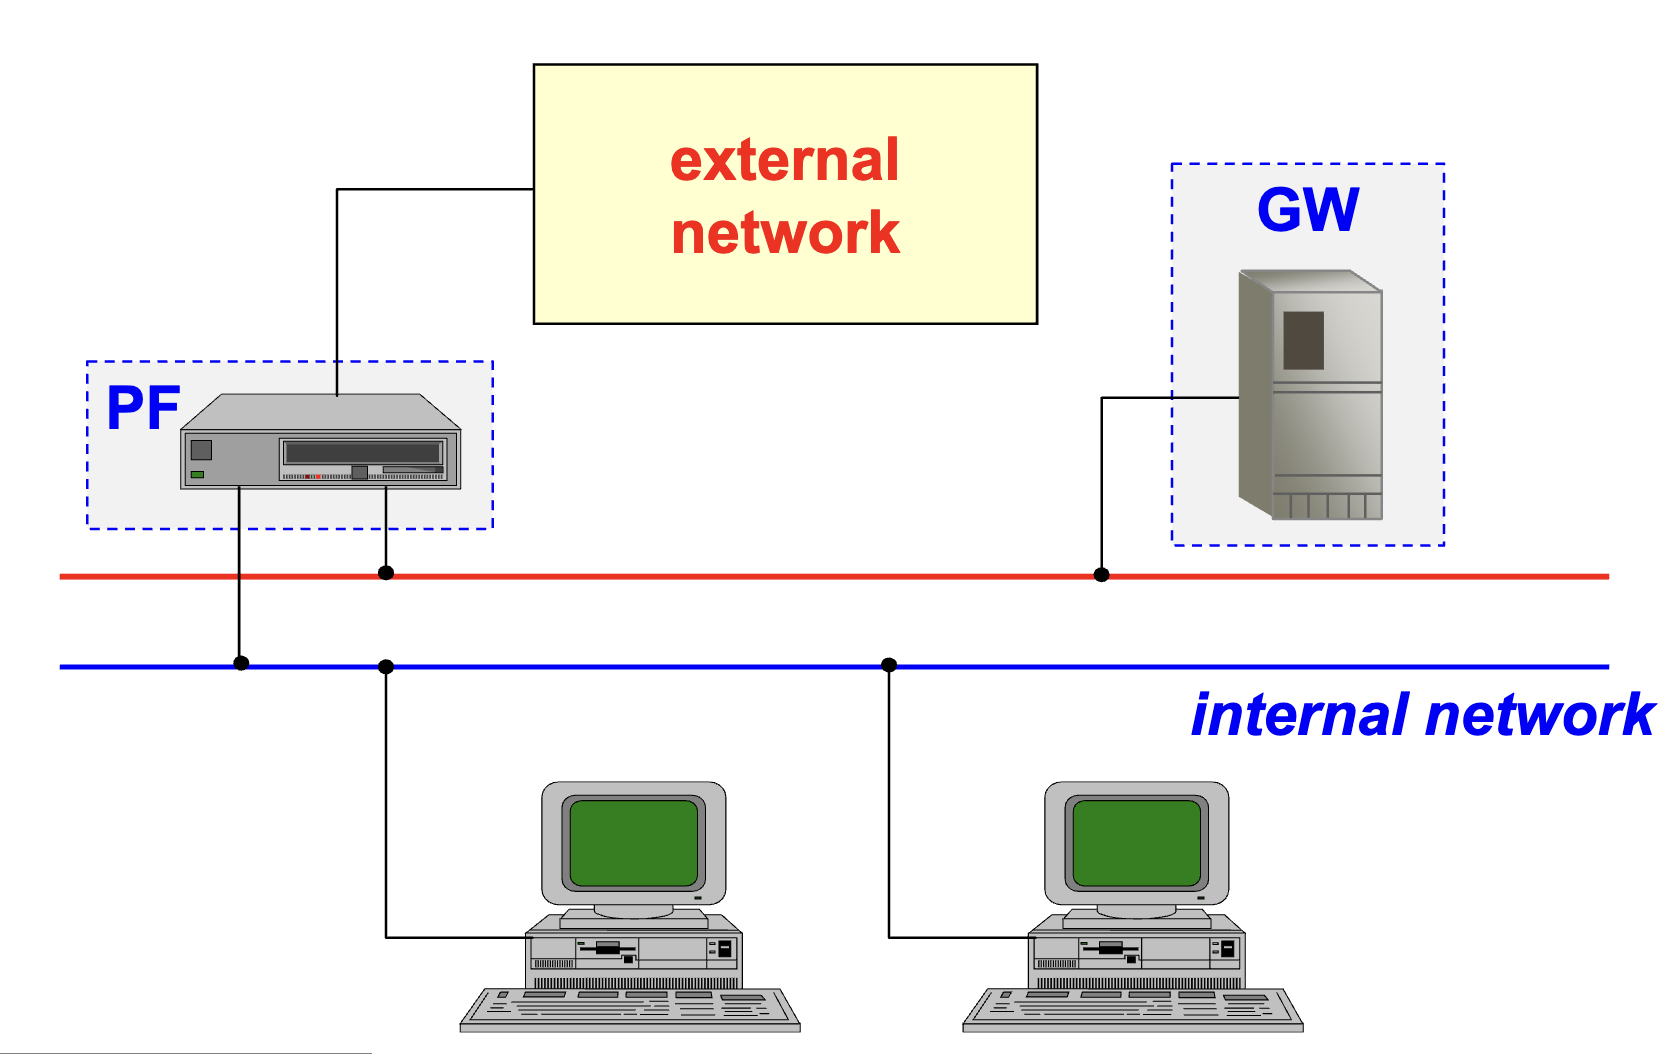
\includegraphics[width=0.5\linewidth]{Images/Firewalling/screened_host.png}
    \caption{Screened host architecture.}
\end{figure}

\subsection{Screened Subnet}
\textcolor{blue}{The most secure solution}, however very complex and expensive. Creates a buffer zone between an internal network and an external network (such as the internet). The screened subnet typically involves two firewalls and a DMZ (Demilitarized Zone) to filter and control the flow of data between the internal network and external network. This setup ensures that external entities can access certain resources without directly exposing the internal network, providing an additional layer of security.

\begin{tcolorbox}[colback=red!10!white, colframe=red!70!black, coltitle=white, title=Beware]
The bastion host must not be in the internal network.

\hfill 

The two packet filters should not have the same implementation (i.e., they should not be from the same vendor).
\end{tcolorbox}

\begin{tcolorbox}[colback=blue!10!white, colframe=blue!50!white, title=DMZ]
    The De-Militarized Zone (DMZ) is home not only to the gateway but also to other hosts, typically the public-facing servers.
\end{tcolorbox}

\begin{figure}[H]
    \centering
    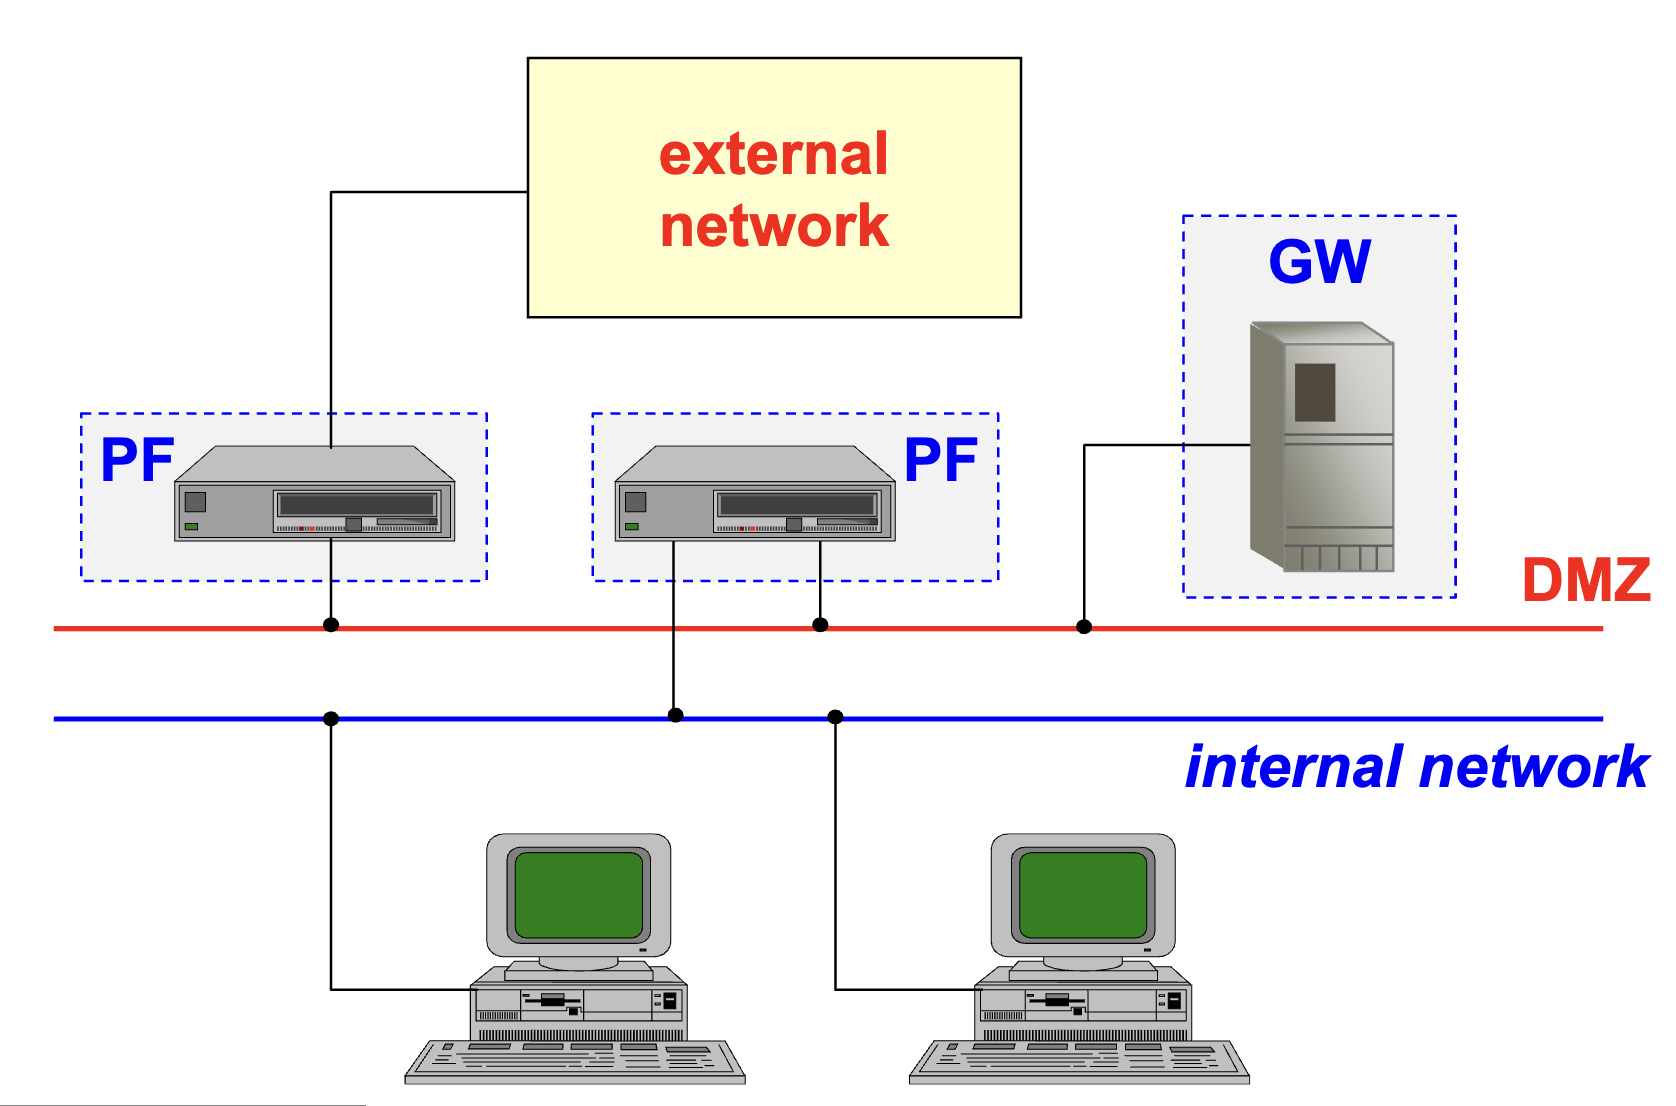
\includegraphics[width=0.5\linewidth]{Images/Firewalling/screened_subnet.png}
    \caption{Screened subnet architecture.}
\end{figure}

\subsection{Screened Subnet V2}
\begin{center}
    (AKA Three-Legged Firewall)
\end{center}

\noindent In this version of the \textbf{Screened Subnet} architecture, the \textbf{packet filter (PF)} and \textbf{gateway (GW)} functions are often combined into a single device. This version is cheaper but still presents a single point of failure.

\hfill 

\noindent\textbf{Three-Legged Design}: This setup involves a firewall device with three network interfaces.
\begin{itemize}
    \item One interface connecting to the \textbf{external network} (untrusted),
    \item One interface connecting to the \textbf{internal network} (trusted),
    \item One interface connecting to the \textbf{DMZ} (where public-facing services reside).
\end{itemize}

\begin{figure}[H]
    \centering
    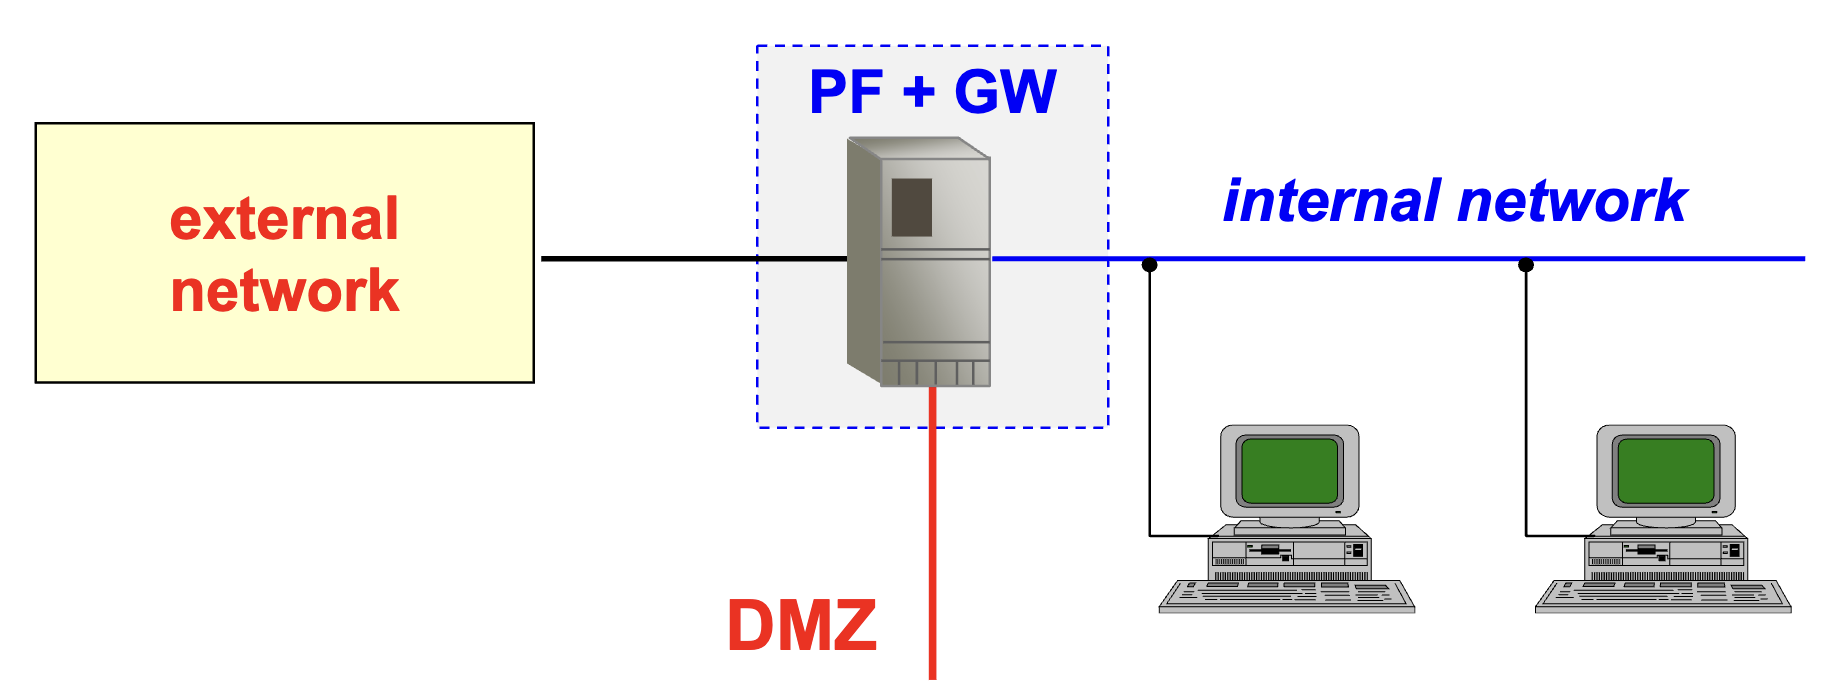
\includegraphics[width=0.5\linewidth]{Images/Firewalling/screened_subnet_v2.png}
    \caption{Three-legged architecture.}
\end{figure}





%-------





\section{Local and Personal Firewall}
Is a firewall (typically, a packet filter) installed directly on the device or server to be protected.

\[
Local \rightarrowtail Server \\
\]

\[
Personal \rightarrowtail User\ Device
\]
Key points:
\begin{itemize}
    \item Differs from network firewalls, which are typically installed at the network perimeter. In fact, my limit the processes that are permitted:
    \begin{itemize}
        \item It can limit processes opening network channels (acting as a client).
        \item It can limit processes answering network requests (acting as a server).
    \end{itemize}
    \item It is usually implemented as a packet filter, controlling the data packets sent to and from the protected device.
    \item Security Goals:
    \begin{itemize}
        \item Helps limit malware and Trojan diffusion within the device or network.
        \item Reduces the risk of configuration mistakes that might expose vulnerabilities.
    \end{itemize}
\end{itemize}

\begin{tcolorbox}[colback=red!10!white, colframe=red!70!black, coltitle=white, title=Beware]
    For the firewall to remain effective, its management must be separate from system management. This separation prevents unauthorized users or processes from tampering with firewall settings.
\end{tcolorbox}

\begin{figure}[H]
    \centering
    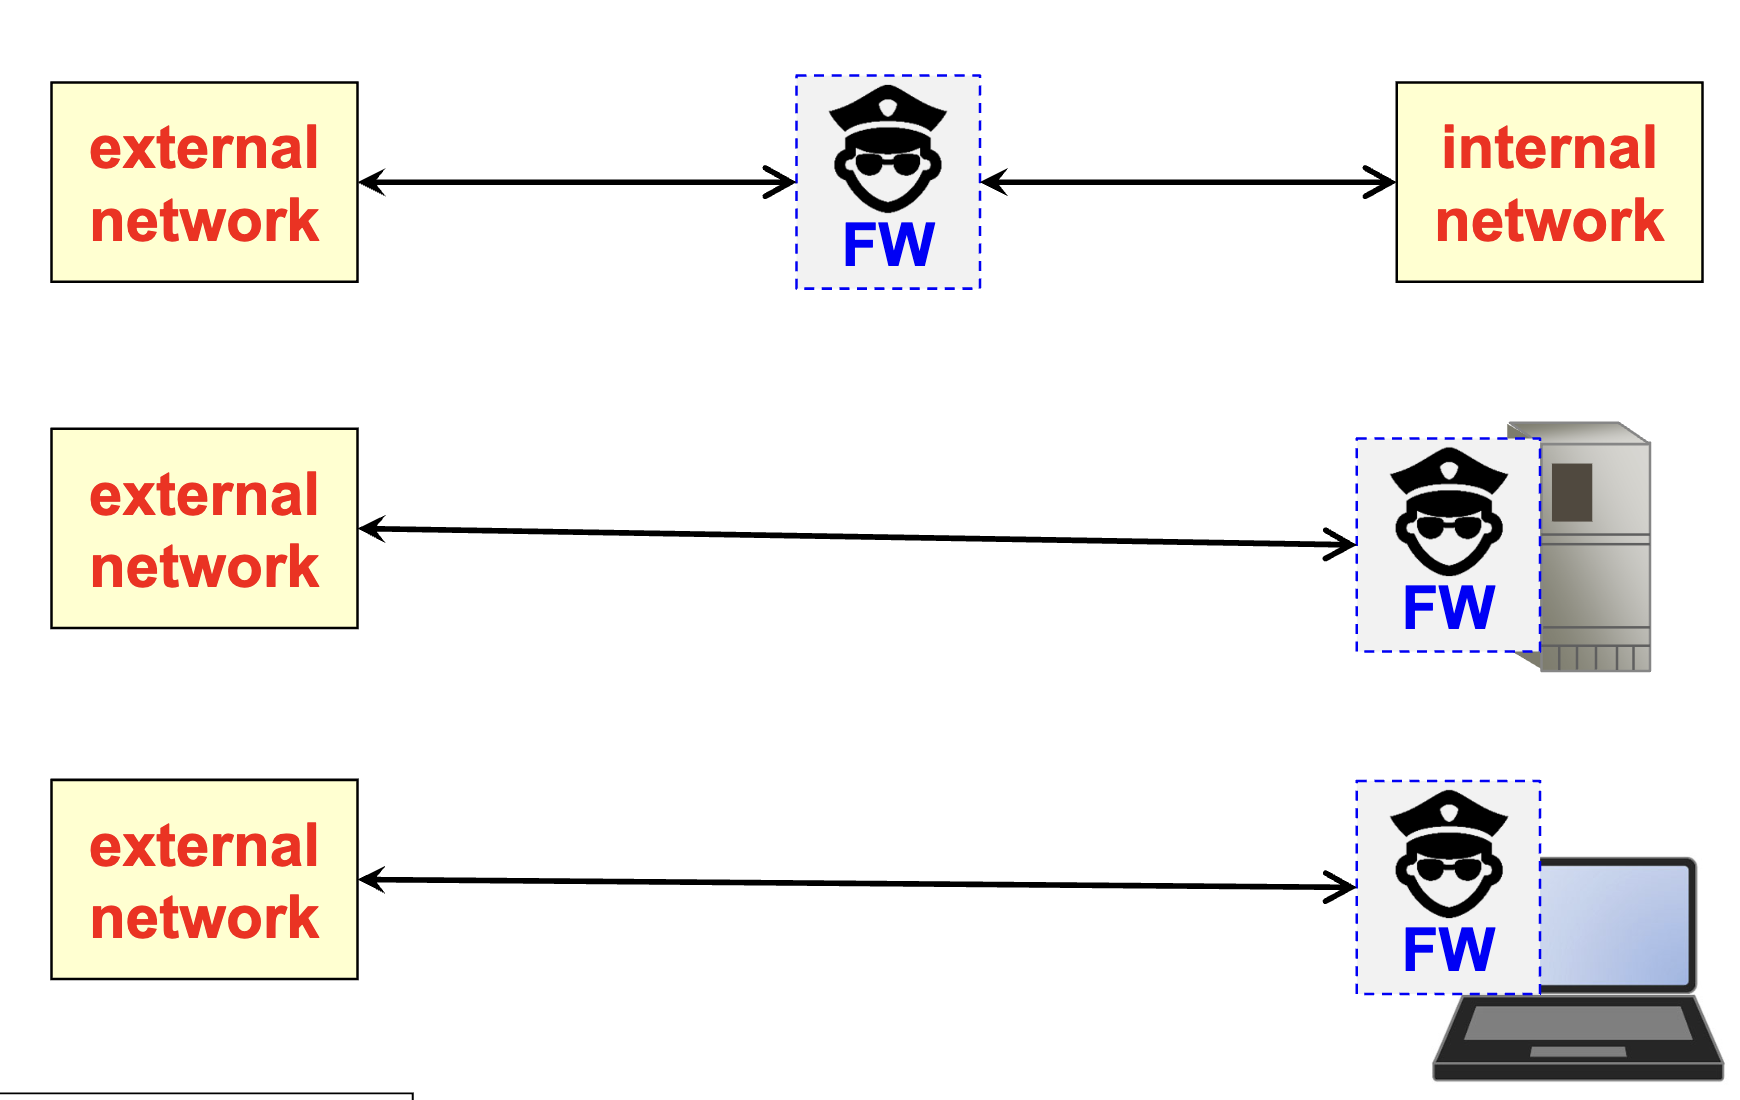
\includegraphics[width=0.7\linewidth]{Images/Firewalling/local_personal_firewall.png}
    \caption{Network, Local and Personal firewall.}
\end{figure}

\section{Firewall Security Features}
This section explains the protection scope and limitations of a firewall:
\begin{itemize}
    \item Effectiveness of a Firewall:
    \begin{itemize}
        \item A firewall is fully effective only against attacks targeting blocked channels (e.g., ports or IP ranges that it is configured to deny).
        \item \textcolor{Red}{Be aware! }It cannot protect against threats coming through allowed channels, as those are intentionally left open for communication.
    \end{itemize}
    \item For the channels left open, other security measures are required to handle potential threats:
    \begin{itemize}
        \item VPN (Virtual Private Network)
        \item Semantic Firewalls or IDS (Intrusion Detection Systems): Analyzes the meaning or behavior of traffic to detect and block malicious activity.
        \item Application-Level Security: Protects specific applications by adding layers of security (e.g., input validation, authentication mechanisms).
    \end{itemize}
\end{itemize}

\subsection{IDS}
\begin{center}
    (Intrusion Detection System)
\end{center}

An IDS is a security system designed to detect:
\begin{itemize}
    \item Unauthorized users attempting to access a system or network.
    \item The actions of unauthorized users within the system.
\end{itemize}

It can also be extended to identify authorized users who violate their privileges, such as accessing data or performing actions beyond their granted permissions.

\hfill

\begin{multicols}{2}
    Core assumption:

    \columnbreak

    \raggedleft
    \textbf{Unauthorized users exhibit different behavioral patterns compared to authorized ones.}
\end{multicols}

\textbf{Functional features:}
\begin{itemize}
    \item Passive IDS:
    \begin{itemize}
        \item Focuses on detection without direct interaction or intervention.
        \item Effect Detection: Identifies the impact of an attack, such as file changes detected through tools like cryptographic checksums or Tripwire.
        \item Pattern Matching: Compares traffic or payloads against known attack or malware signatures to identify threats.
    \end{itemize}
    \item Active IDS:
    \begin{itemize}
        \item Takes a more dynamic and proactive approach to intrusion detection through the following processes.
        \begin{itemize}
            \item Learning: Uses statistical analysis to understand and establish baseline system behavior over time.
            \item Monitoring: Actively collects statistical information about traffic, data flows, sequences, and user actions.
            \item Reaction: Compares real-time activity against the established statistical parameters. Initiates a reaction or alert when certain thresholds (e.g., anomalous traffic or behavior) are exceeded.
        \end{itemize}
    \end{itemize}
\end{itemize}

\begin{tcolorbox}[colback=blue!10!white, colframe=blue!50!white]
    Usually, we have a hybrid strategy, combining both passive and active approaches, and we need a bit of tolerance for false positives to ensure potential threats are not overlooked.
\end{tcolorbox}

\textbf{Topological features:}
\begin{itemize}
    \item HIDS (Host-Based IDS): 
    \begin{itemize}
        \item Operates on individual hosts (e.g., servers, workstations).
        \item Log Analysis: Examines logs generated by the operating system (OS), services, or applications to detect suspicious activities or patterns.
        \item Internal OS Monitoring Tools: Uses tools within the OS to track file integrity, process activity, and other host-level indicators of compromise.
    \end{itemize}
    \item NIDS (Network-Based IDS)
\end{itemize}

\subsubsection{NIDS}
\begin{center}
    (Network-Based IDS)
\end{center}
Monitors and analyzes network traffic across a network segment or the entire network. Uses Network Traffic Monitoring Tools, which capture and examine packets flowing through the network to detect unusual patterns, malicious payloads, or unauthorized access attempts.

\textbf{Components:}
\begin{itemize}
    \item Sensor: The sensor is responsible for monitoring network traffic and logs to detect potential security threats.
    \begin{itemize}
        \item Traffic and Log Analysis: It scans the network traffic and logs for suspect patterns that might indicate an attack or malicious activity.
        \item Security Event Generation: When suspicious patterns are detected, the sensor generates security events to report them.
        \item Interaction with the System: The sensor can take actions based on detected threats, such as modifying Access Control Lists (ACLs) or triggering a TCP reset to disrupt a malicious connection.
    \end{itemize}
    \item Director: The director is the central component that coordinates and manages the NIDS system.
    \begin{itemize}
        \item Sensor Coordination: It manages the interaction and operation of multiple sensors distributed across the network.
        \item Security Database Management: The director manages a database that stores security events, logs, and configurations for future analysis and reporting.
    \end{itemize}
    \item  IDS Message System: This component ensures secure and reliable communication between the various NIDS components (sensors, director, etc.).
    \begin{itemize}
        \item It ensures that data and alerts are transmitted between components securely, preventing tampering or loss of critical information.
    \end{itemize}
\end{itemize}

\noindent\textbf{Architecture:}

The workflow of a Network-Based Intrusion Detection System (NIDS) architecture involves several steps (fig.\ref{fig:nids_architecture}):
\begin{itemize}
    \item Sensors:
    \begin{itemize}
        \item Capture network traffic (packets) and log information from various points within the network.
        \item Compare the network traffic and logs to a set of predefined attack signatures or anomaly patterns.
    \end{itemize}
    \item Anomaly Detection: If the traffic deviates from normal behavior, the sensor may identify it as an anomaly (e.g., a DDoS attack, port scanning, or other unauthorized access attempts).
    \item If suspicious activity is detected, the sensor generates security events and sends them to the IDS director.
    \item The director analyzes and correlates incoming events from multiple sensors, looking for patterns or sequences of activities that indicate a more significant attack (e.g., a coordinated attack across multiple sensors).
    \item Immediate Actions: Based on predefined rules, the director can initiate automatic responses.
\end{itemize}

\begin{figure}[H]
    \centering
    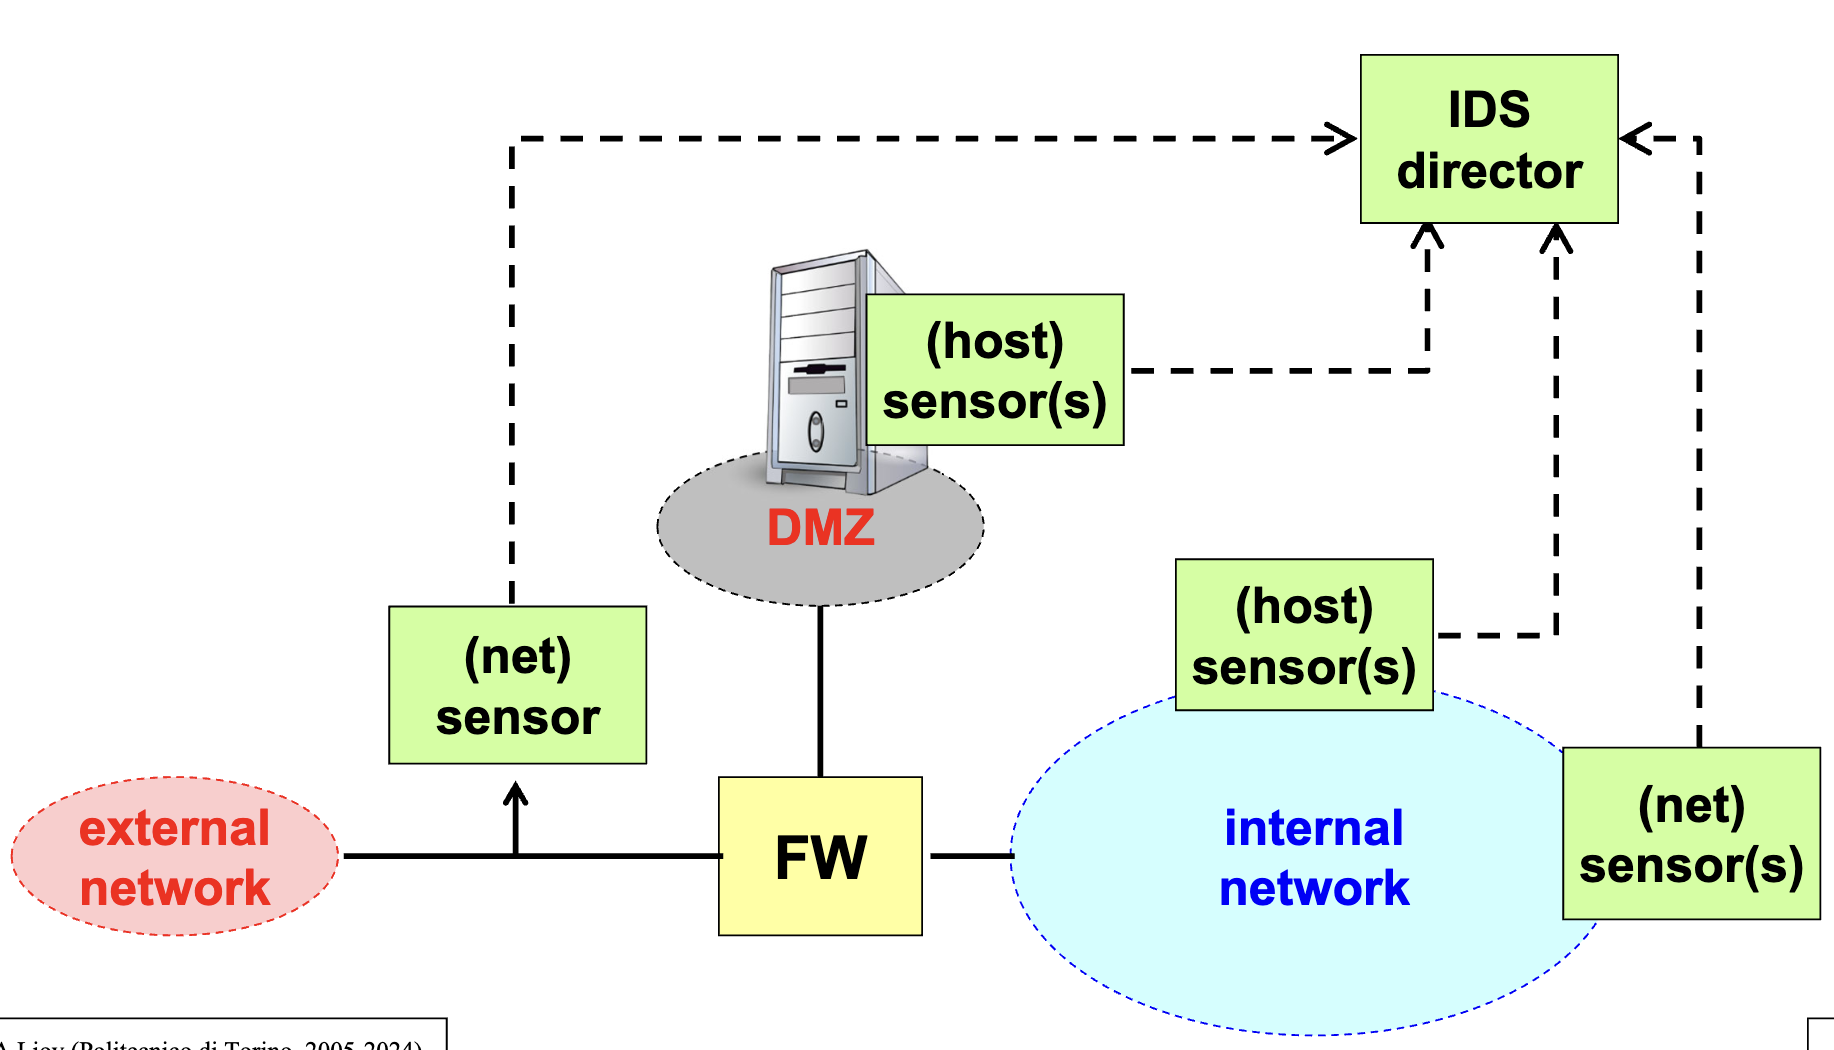
\includegraphics[width=0.7\linewidth]{Images/Firewalling/nids_architecture.png}
    \caption{Network-based IDS architecture.}
    \label{fig:nids_architecture}
\end{figure}

\section{Other Firewall Implementations}

\subsection{IPS}
\begin{center}
    (Intrusion Prevention System)
\end{center}

An IPS combines Intrusion Detection with the capability to actively prevent detected threats. The goal is to speed up and automate the response to intrusions by integrating an IDS (Intrusion Detection System) with a distributed dynamic firewall, which can take immediate actions to block malicious traffic.

\begin{tcolorbox}[colback=red!10!white, colframe=red!70!black, coltitle=white, title=Beware]
Dangerous! IPS systems can erroneously block or allow traffic, potentially causing harm to the network or users if the wrong decision is made.
\end{tcolorbox}

\begin{itemize}
    \item An IPS is not just a standalone product; it’s a technology that can be integrated into the overall security infrastructure to provide real-time detection and mitigation of attacks.
    \item Many modern security systems integrate IDS and IPS into a single product known as IDPS (Intrusion Detection and Prevention System).
\end{itemize}

\subsection{NGFW}
\begin{center}
    (Next-Generation Firewall)
\end{center}

Extends traditional firewall functionality by integrating advanced features that provide deeper inspection and more granular control over network traffic. 

Key features:
\begin{itemize}
    \item Application Identification: 
    \begin{itemize}
        \item Can identify and control applications regardless of the port or protocol used (w.r.t. classic firewalls an NGFW analyzes also traffic patterns on the application layer).
        \item Deciphering/Re-ciphering Traffic: NGFWs can perform SSL/TLS decryption to inspect encrypted traffic, allowing them to detect hidden threats in secure communications.
    \end{itemize}
    \item User Identification:
    \begin{itemize}
        \item NGFWs can integrate with user authentication mechanisms, enabling them to enforce policies based on the user rather than just IP addresses.
        \item Integration with: Captive Portals (e.g., Wi-Fi), 802.1x and end-point authentication (e.g., Kerberos, Active Directory, and LDAP)
    \end{itemize}
    \item Per-User and Per-Application Policies:allow the creation of security policies that are user-specific and application-specific (For example, an NGFW could block social media applications for some users while allowing them for others).
    \item Filtering based also upon known vulnerabilities, threats, malware
\end{itemize}

\subsection{UTM}
\begin{center}
    (Unified Threat Management)
\end{center}
Integrates multiple security functionalities into a single device. This approach simplifies network security by combining various protections into one solution, making it easier to manage and often more cost-effective.

\hfill 

Key features:
\begin{itemize}
    \item Common capabilities: firewall, VPN, anti-malware, content-inspection, IDPS (Intrusion Detection and Prevention System).
    \item Actual capabilities depend upon the manufacturer.
    \item Mainly targeted to reduce the number of different systems,
    hence the management complexity and the cost
\end{itemize}

\subsection{Honey Pot / Honey Net}
Security tools designed to deceive attackers by creating artificial environments that simulate vulnerable systems or networks. Their main purpose is to attract and observe malicious activity, helping security professionals gather information on attack methods, identify vulnerabilities, and develop better defense strategies.

\begin{figure}[H]
    \centering
    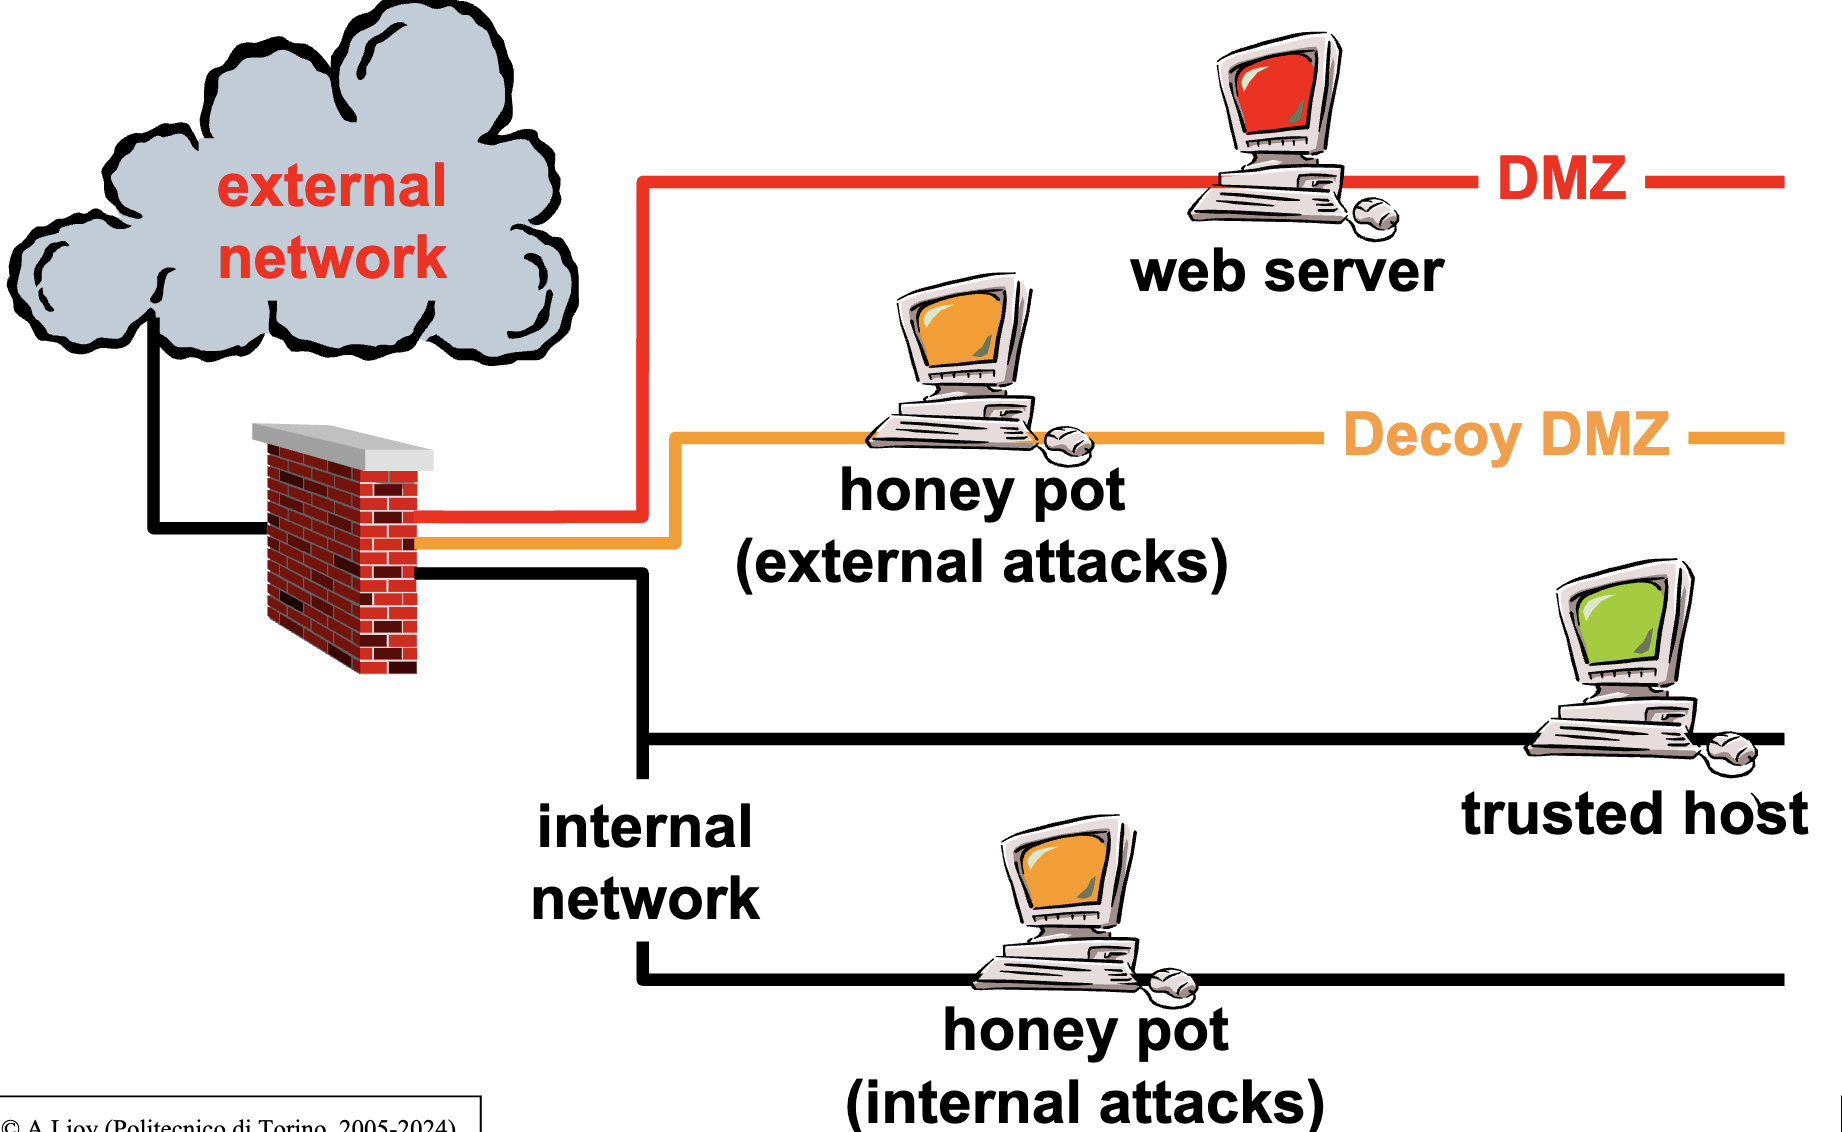
\includegraphics[width=\linewidth]{Images/Firewalling/honey_pot.png}
    \caption{Honey pot architecture.}
\end{figure}